\chapter{Design}



%You should concentrate on the more important aspects of the design. It is essential that an overview is presented before going into detail. As well as describing the design adopted it must also explain what other designs were considered and why they were rejected.

%The design should describe what you expected to do, and might also explain areas that you had to revise after some investigation.

%Typically, for an object-oriented design, the discussion will focus on the choice of objects and classes and the allocation of methods to classes. The use made of reusable components should be described and their source referenced. Particularly important decisions concerning data structures usually affect the architecture of a system and so should be described here.

%How much material you include on detailed design and implementation will depend very much on the nature of the project. It should not be padded out. Think about the significant aspects of your system. For example, describe the design of the user interface if it is a critical aspect of your system, or provide detail about methods and data structures that are not trivial. Do not spend time on long lists of trivial items and repetitive descriptions. If in doubt about what is appropriate, speak to your supervisor.


\section{Overall Architecture}
The initial design for the robot is to produce a small vehicle capable of moving freely within an environment under it's own power with a platform for mounting the various systems.  These systems should be a central control unit, motor control and the various sensors.

\begin{figure}[H]
\centering
        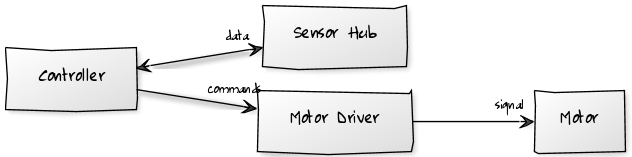
\includegraphics[width=4.0in] {Images/basic-uml.png}
        \caption{Basic system diagram}
        \label{Basic system diagram}
\end{figure}


\begin{figure}[H]
\centering
        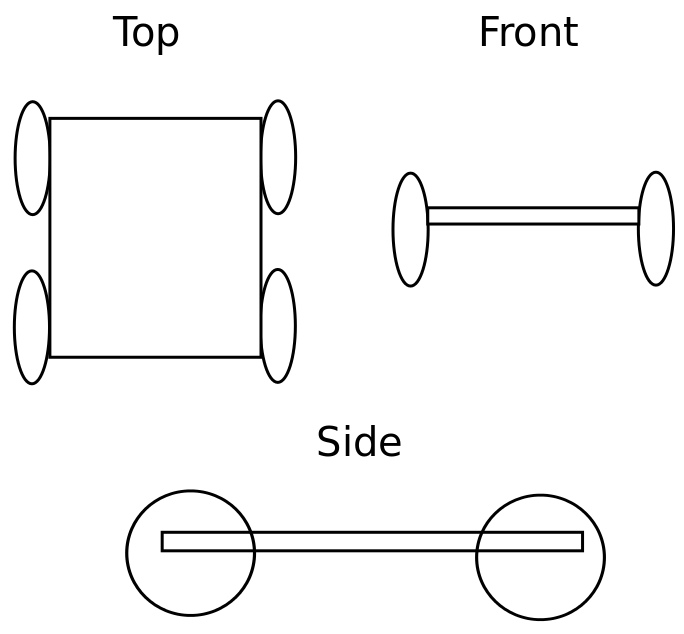
\includegraphics[width=2.0in] {Images/initial-design.png}
        \caption{Initial design}
        \label{Initial design}
\end{figure}

The central control unit will be a microcontroller for ease of interfacing directly with hardware as well as keeping power consumption down.  Keeping power consumption to a minimum is important so that the robot can be active for a longer period of time without needing to be recharged.  This controller will interface with both a motor control system and the various sensors required to detect objects in the environment local to the robot.

\section{Design Research}
The various components that the project will need to come together into a finished product have many different possible options to choose from, all with their various strengths and weaknesses.
\subsection{Materials}
There were several considered materials for the robot chassis to be built of and the ideal material would be:
\begin{enumerate}
\item Extremely difficult to break so that it does not get damaged easily while in use.
\item As light as possible to make it easier on whichever drive system is used to move it.
\item To be as low cost as possible so that it is affordable to a student.
\item Something that does not conduct electricity which could possibly damage an electrical component mounted onto it.
\item Hard to bend to avoid being bent out of shape by any possible heavy load the robot may end up carrying or colliding with.
\item Easy to cut so that it is possible to craft into the required shape.
\end{enumerate}

\begin{itemize}
\item Wood
\\This would be the easiest material to make the chassis from as it is very cheap, easy to cut into the intended shape and easy to mount components on with either adhesive, nails or screws.  Also the fact that it does not conduct electricity will help when mounting circuit boards to it.

\item Plastic
\\The lightest option.  Good due to its low weight but may not be as strong as wood or a metal option and could bend or snap under the load of heavier components such as motors or a large power source.  It can be more expensive than wood to acquire.  There is a higher difficulty in cutting it into the desired shapes.  It is also non-conductive, again useful to mount electronic components to.  Plastic can hold a static charge which can be damaging to electrical components.

\item Steel
\\A stronger material that can withstand a much heavier load than wood of plastic. It may be able to withstand a heavier load before it is bent out of shape but is itself more heavy than the weaker options of wood or plastic.  This extra base weight before adding anything else will put more strain onto which ever drive system that is used to drive the robot and may even need to use more powerful motors because of this extra weight.  It is a very conductive material which means that a non-conductive mounting platform will also be needed to mount electronic components as to avoid damaging them.

\item Aluminium
\\A much lighter metal than steel, but still much heavier than wood or plastic or the same thickness.  It can also withstand heavier loads than wood or plastic but it also much more difficult to cut.  Again aluminium is a very conductive material meaning that a non-conductive mounting platform will be needed.  It can also be used as a heat sink for the components that can get very hot such as the motor drivers or the motors themselves.  A heatsink is a material attached to something that gets very hot and conducts that heat.  It generally has a large surface area to dissipate the heat into the cooler air around it, but it may also have a fan to blow/draw the hotter air away replacing it with air/gas with a lower temperature than that of the heatsink.

\end{itemize}

Aluminium seems to be the best all round choice being strong but not as heavy as steel.  It can act as a heat sink if the motors are mounted directly to it.  It is also not very expensive to buy in small amounts.
\\In addition to the aluminium base I have decided to use plastic for mounting components to the base as it is light, inexpensive and non conductive which is suitable for electronic components.

\subsection{Actuators}
Actuators are motors used for controlling movement of a system.  The ideal actuator would be something that:
\begin{enumerate}
\item Has little to no power consumption which will increase the overall total runtime of the robot by decreasing the energy draw on the system.
\item Has as much torque as possible to make moving a larger mass less effort.
\item Weighs as little as possible to reduce the overall weight of the robot.
\item Is as low cost as possible again to be affordable to a student building this robot.
\item Has perfect precision in order to know exactly what position it is in at any time.
\item Have no limits on rotation as some actuators can only turn a set amount before having to turn back.
\item High speed range so that it can move as slow as needed or as fast as needed.
\item No wear and tear for easy or no maintenance.
\end{enumerate}
\begin{itemize}
\item Servo
\\Typical servos are a motor and a gearbox with a potentiometer, a voltage divider in this case used to determine how far a motor has turned, for feedback.  These motors are great for controlling such things as the direction of sensors or moving very light devices.  Servos are low voltage, typically 4.8 - 6 volts, and as such do not have much strength, which means that they are typically not good for driving larger equipment.  Additionally most servos only turn up to 180 degrees or 360 degrees.  In normal operation they do not turn continuously but can be modified to do so at the cost of losing the feedback of how far the motor has turned.
\begin{figure}[H]
\centering
        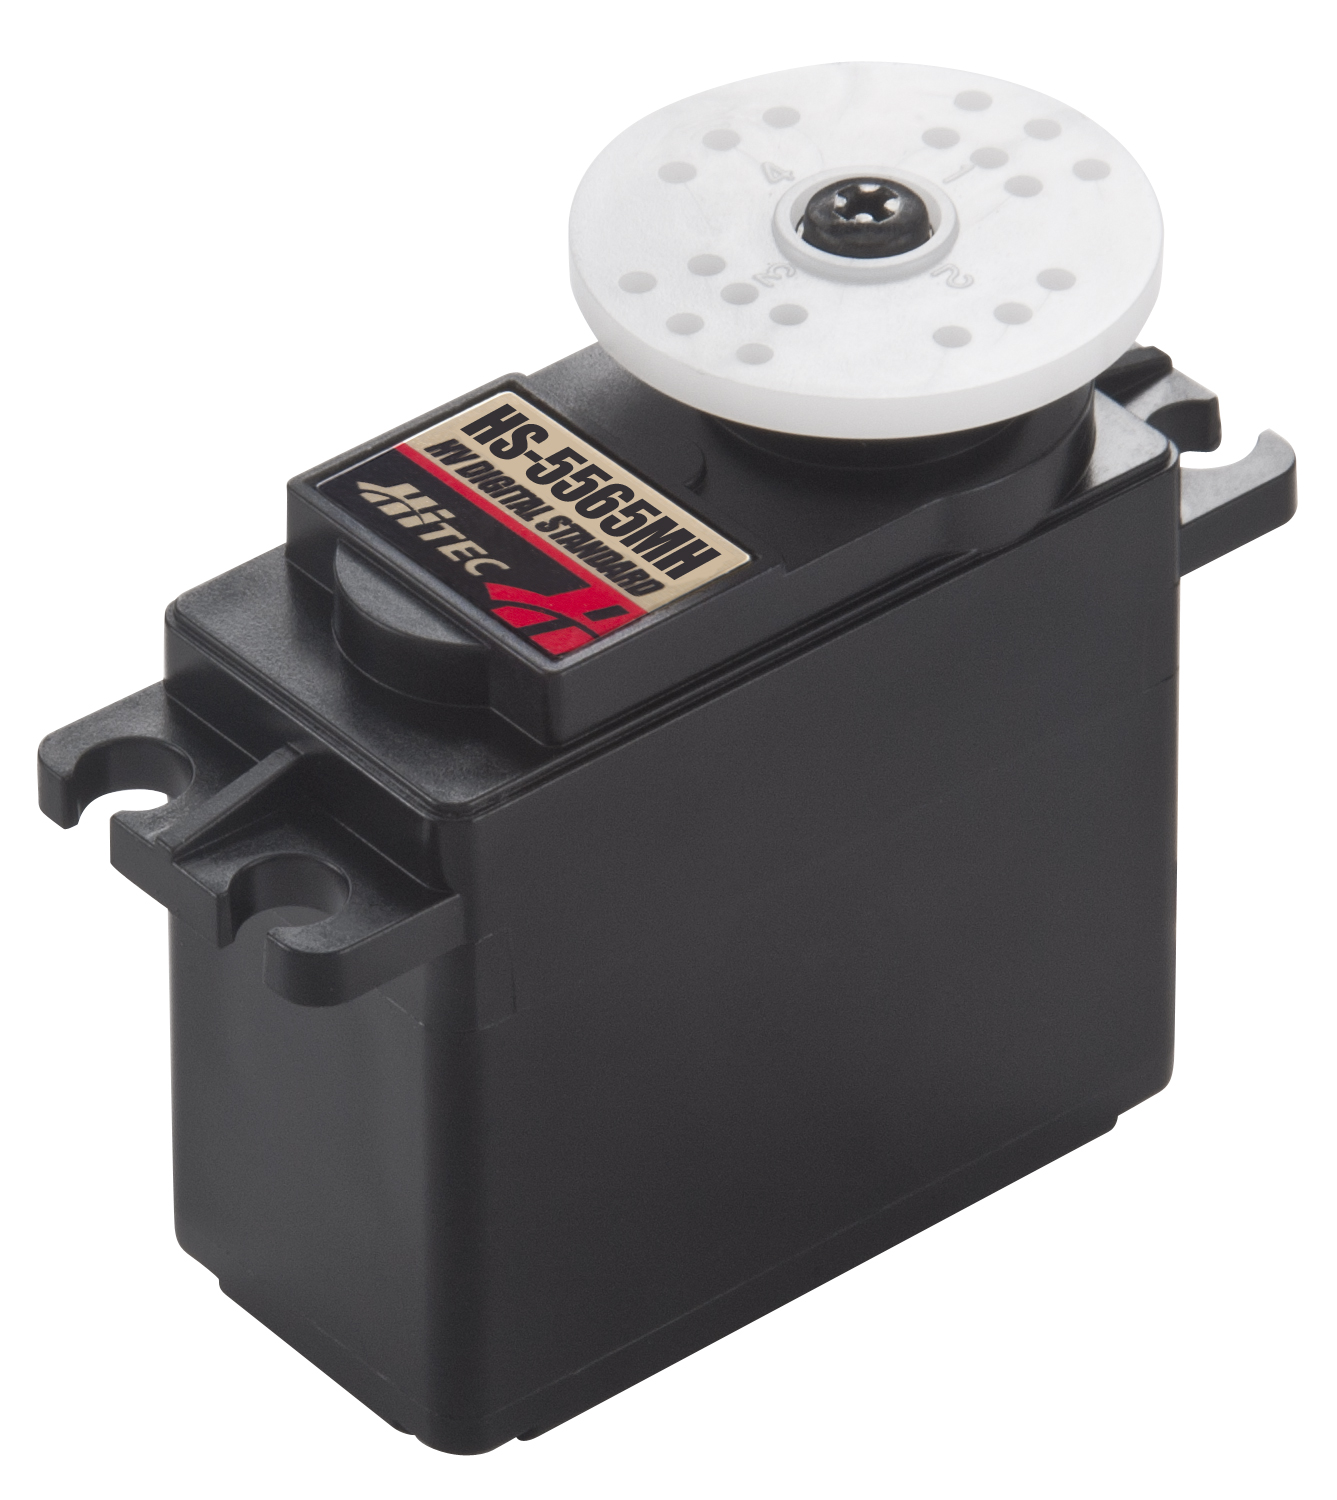
\includegraphics[width=1.5in] {Images/servo.jpg}
        \caption{Servo Motor - robotshop.com}
        \label{Servo Motor}
\end{figure}

\item DC Motor
\\Direct current motor has a very simple operation: apply current to one side of the motor to make it turn, reverse the direction of the current to reverse the direction the motor turns.  Changing the speed of these motors is simple, either change the voltage (keeping it within the devices tolerances) or turn the current supplied to the motor on and off at high speed where how quickly it is alternated determines the speed of the motor.  Typically these motors are attached to a gearbox to gain more torque to drive much higher loads.  Optical rotary encoders can be used to determine how much the motors have turned and how fast.  An optical rotary encoder can be fitted to any motor to add the functionality of positional feedback.  These encoders use a light based sensor to detect when the light changes in front of it, this can be used with a disc that has black and white lines on it.  The change in color is detected, this along with how many times it changes and with what frequency this happens can determine the amount a wheel has turned and how fast it has done so.
\begin{figure}[H]
\centering
        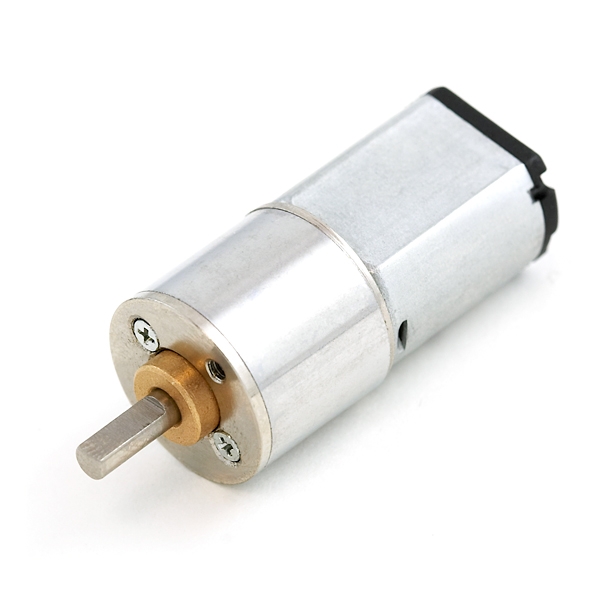
\includegraphics[width=2.0in] {Images/dc-motor.jpg}
        \caption{DC Motor - sparkfun.com - CC BY-NC-SA 3.0}
        \label{DC Motor}
\end{figure}
\item Steppers
\\Stepper motors use an internal gear and a ring of magnets.  These magnets pull the gear into position, powering the magnets in sequence which will turn the motor.  Each part of this cycle is called a step.  This means that a single step is a known amount of rotation.  Using this type of motor ensures that you can accurately turn whatever is attached to the motor shaft by a known amount without any additional measuring equipment.  But adding any such measuring equipment can add verification to determine if the motor has actually rotated by the amount expected.
\begin{figure}[H]
\centering
\begin{subfigure}
	\centering
        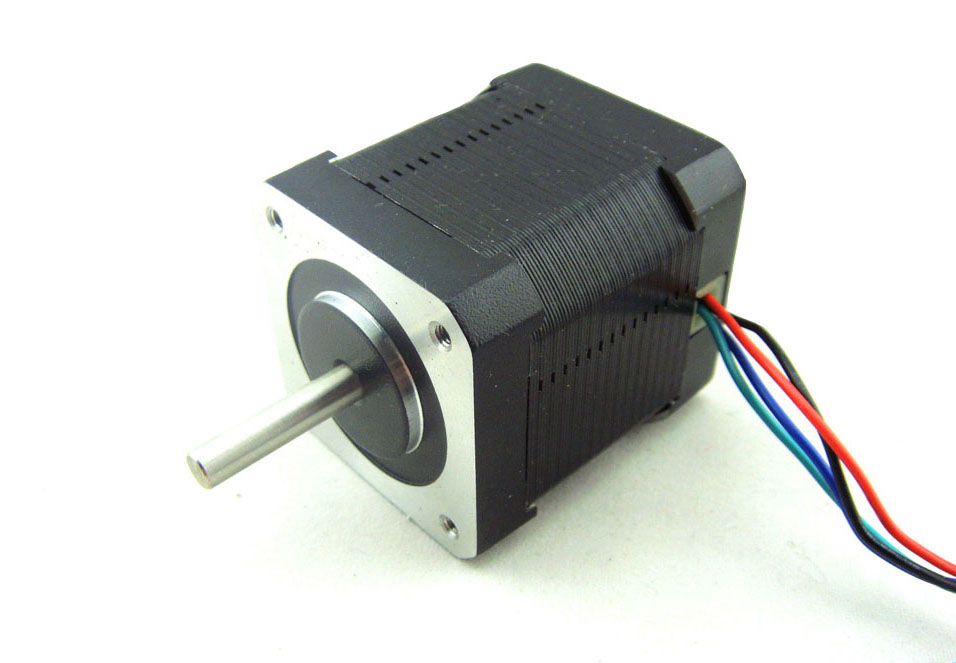
\includegraphics[width=2.0in] {Images/stepper.jpg}
        \caption{Stepper Motor - stepperonline.com}
        \label{Stepper Motor}
\end{subfigure}
\begin{subfigure}
        \centering
        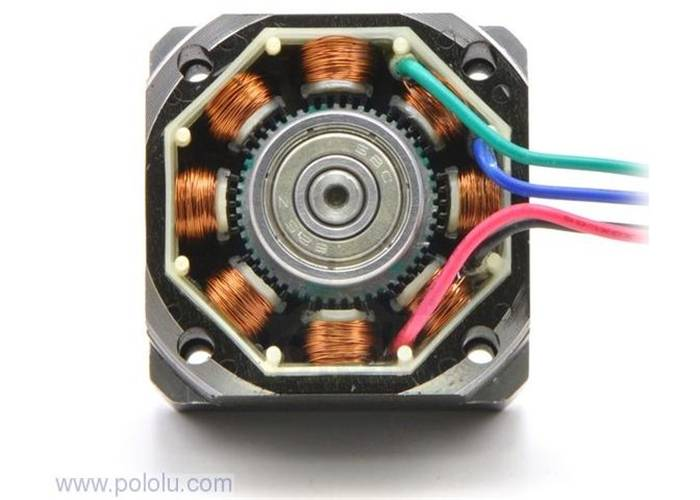
\includegraphics[width=2.0in] {Images/stepper-internal.jpg}
        \caption{Stepper Motor Internal- robotgear.com.au}
        \label{Stepper Motor Internal}
\end{subfigure}
\end{figure}
\end{itemize}

I have chosen to use stepper motors due to the ability to control the amount and speed of rotation with more accuracy than the alternatives.  Stepper motors do come in high torque version which may be needed for this project as the chassis is made of metal which is a much heavier material.  A stepper motor could be used with a chassis of any of the materials mentioned, it may struggle with steel depending on how thick of a piece is used.  DC motors could also be used with all materials if in conjunction with a gearbox, but the additional system needed to measure and control the exact rotation of the wheels using this method puts me off of the idea.  Greater power but less accurate control.
\subsection{Drive Type}
There are various different ways to move a mass around.  The ideal drive system should be:
\begin{enumerate}
\item A very low mass to reduce overall load on the system.
\item Capable of omni-directional movement to increase the ease of moving within confined environments.
\item Perfectly stable so that the robot doe snot fall over or collapse.
\item Have high traction as to not slip on it's environment.
\end{enumerate}
No single drive system is going to be perfect in all aspects.
\begin{itemize}
\item Wheels
\\These are most conventional method of movement which are seen by most people every day.  Robots that use wheels to enable movement are often very stable and can be using in many configurations.
	\begin{itemize}
	\item Two Wheels
	\\This is an unstable configuration which requires it to be in constant motion to maintain an upright position.  When configured with the wheels side by side the center of gravity will be directly in the middle between the wheels underneath the axle where a weight is often positioned to help keep it upright as well as a tilt sensor to help compensate for movement.
\begin{figure}[H]
\centering
        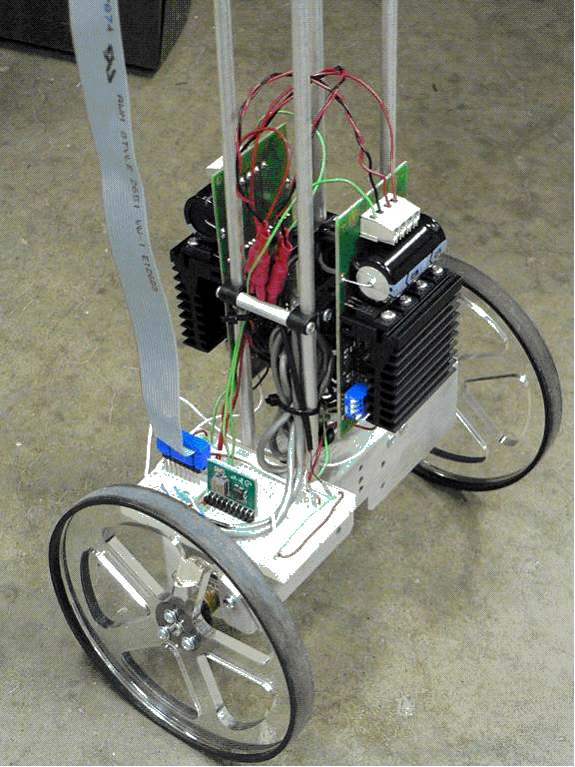
\includegraphics[width=2.0in] {Images/2-wheel-side.png}
        \caption{2 Wheel Gyroscope - ni.com}
        \label{2 Wheel Gyroscope}
\end{figure}
Another way for a two wheels to be arranged would be like a bike where again it will need to be in constant motion to remain upright.


	\item Three Wheels
	\\Most commonly two drive wheels and a single free turning wheel for stability.  To turn the wheels are either turned in the opposite direction of each other or in the same direction just as different speeds using the free turning wheel to stop it falling over or being pulled along the ground as long as the center of gravity if within the three wheels.

	\item Four Wheels
	\\All four wheels can have independent control for tank style movement.  This is harder to keep in a straight line due to having to try and keep all four wheels turning at the same speed otherwise risk being inefficient and also causing additional friction dragging one side back.  An advantage to having all four wheels operated independently is that if using in conjunction with 'omni' wheels.  These wheels have rollers on them enabling then to traverse in a lateral direction if the front and back pair are rotated in the opposite direction of each other.
	\\Car type configuration is also four wheels but only either the front or the back pair are powered and either the front of back pair are able to turn.  Both the wheels that are able to change direction and the powered drive wheels can be the same pair.  It will require some kind of servo system to turn the axis which is designated at the turning wheels.

	\item More than Four Wheels
	\\Very good for uneven terrain as each wheel can rise and fall independently with less effect on the main structure.  These are far more complex to operate but if the terrain is very rocky then it may be the best choice.
	\end{itemize}

\item Tracks
\\These are very stable and have the best traction compared to wheeled variants as long as the surface it is used on is not smooth, sand is a good place to use tracks due to the large surface area compared to wheels as they will not sink while wheels will.  Very high friction with the ground especially when turned as it has to operate the tracks in the opposite direction of each other forcing its way around in a circle.
\begin{figure}[H]
\centering
        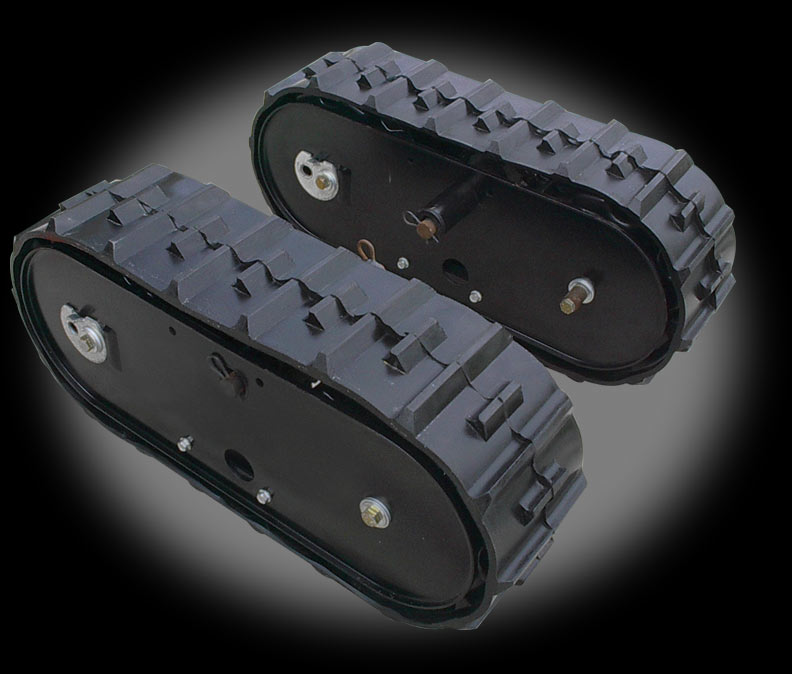
\includegraphics[width=2.0in] {Images/wheel-track.jpg}
        \caption{Tracks - robotcombat.com}
        \label{Tracks}
\end{figure}


\item Legs
\\These are the most uncommon of the movement types.  Due to the cost of developing systems using this type of movement and the overall complexity of controlling them.
	\begin{itemize}
	\item Single Leg
	\\The most difficult to control due to having to balance its load upright on a single point and having to lean in the direction it needs to go without falling over and 'hop' to move around without falling over when landing.
\begin{figure}[H]
\centering
        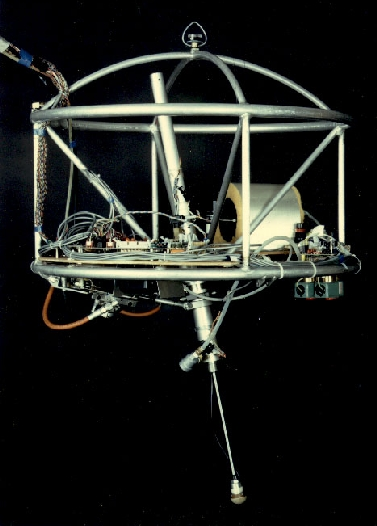
\includegraphics[width=2.0in] {Images/3d-hopper.jpeg}
        \caption{3D One Legged Hopper - mit.edu}
        \label{3D One Legged Hopper}
\end{figure}
	\item Two Legs
	\\Extremely difficult to control and there are very few working practical applications of a two legged robot.  The main issue for controlling this is keeping it upright and not overbalancing, also if knee type joins are added the complexity significantly increases.
	\\Also the mere fact that work on two legged robots is being done by a cutting edge engineering company like Boston Dynamics \cite{boston} is evidence that this kind of system is a fair bit beyond the scope of an undergraduate student project.

\begin{figure}[H]
\centering
        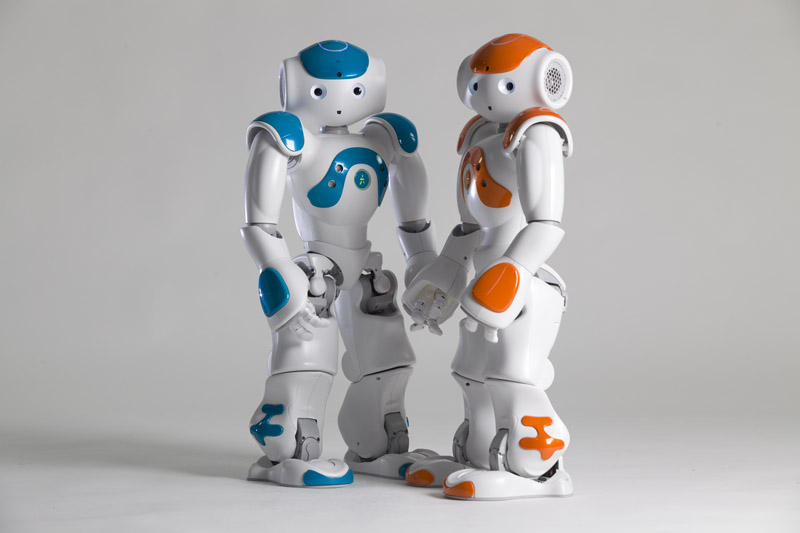
\includegraphics[width=4.0in] {Images/nao.jpg}
        \caption{NAO - aldebaran-robotics.com}
        \label{NAO}
\end{figure}
	\item More than Four Legs
	\\Having more legs can increase stability.  This is because most of the legs can be firmly on the ground while the others are moving into their new position.  Turning can be more complicated to control than the walking already is.  The servos used to control each of these legs and all the joints the legs may have may need to be quite strong or at least have strong teeth as to not get stripped under the weight of whatever payload the robot may have on top of all of these legs.  This is based on how insects are constructed where their body is vastly bigger than its legs, and as such it has many legs to compensate for this and distribute the load.
	\end{itemize}
\end{itemize}
I have decided to use a four wheel configuration to take advantage of the level of traction four wheels will give the robot as well as the added stability over the two or three wheeled configuration.  The configurations with more than four wheels have added complexity in how to control all of the extra wheels and the advantages of having the added wheels are not needed in this project.  Also the legged variety of drive systems are well beyond the scope of this project and the added complexity would not bring any real benefits tot he robot for it's intended purpose of avoiding obstacles in the environment.
\subsection{Sensors}
Sensors are needed so that the robot is able to see what is in the environment around it, enabling it to see, calculate and avoid obstacles.
\\An ideal sensor would be:
\begin{enumerate}
\item Infinite range, being able to see as far as possible and as close as possible.
\item Can no be interfered with, able to be used in any environment and nothing can interfere with the readings it provides.
\item Little to no processing required to acquire and interpret the data provided by the sensor.
\item Lightweight as to not increase load on the drive system.
\item Small so that many can be fitted into a small space for maximum obstacle sensing ability.
\item Cheap as possible to be able to afford many.
\item High resolution as to be able to determine what exactly the objects in the environment are.
\end{enumerate}
Such a wonderful sensor does not exist but there are many options.
\begin{itemize}
\item Bump Skirt
A bump skirt is multiple touch sensors such as buttons arranged like a skirt around the edge of the robot.  When the robot bumps into something the button is pressed telling the robot where it bumped into something.  From this it will be able to move in the appropriate direction to get away from the object it hit.  This is a very bad way of avoiding an obstacle because to know that something is there it will have to hit it first.

\item LDR
\\An LDR is a light dependant resistor.  A small resistor that changes its resistance depending on how much light it is exposed to.  This could be used to detect if the robot is very close to bumping into an object and avoid it as the object got closer and possibly cast a shadow onto the sensor reducing the amount of light the resistor can detect, similar to a physical bump skirt which activates when something touches it.
\begin{figure}[H]
\centering
        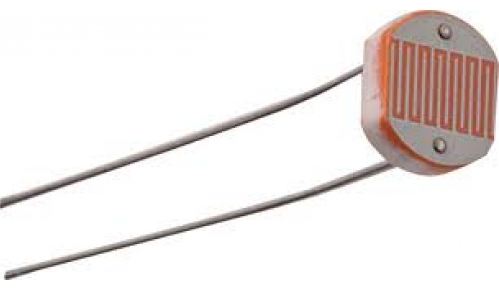
\includegraphics[width=2.0in] {Images/ldr.jpg}
        \caption{Light Dependant Resistor - robotics.org.za}
        \label{Light Dependant Resistor}
\end{figure}

\item Camera
\\A camera could be used to detect objects in front of it by using various image processing techniques to analyse the data it provides.  This method is good because it can potentially map a relatively large area in a single image.  However it requires more processing to do so, which can be slow and result in colliding into an object or being stuck in a tight space before the system has finished processing data from the camera.  This method would force me to use a more powerful processor to overcome the limits of the lower speed processor models but it adds complexity to the project as well as additional cost and a higher power consumption.
\begin{figure}[H]
\centering
        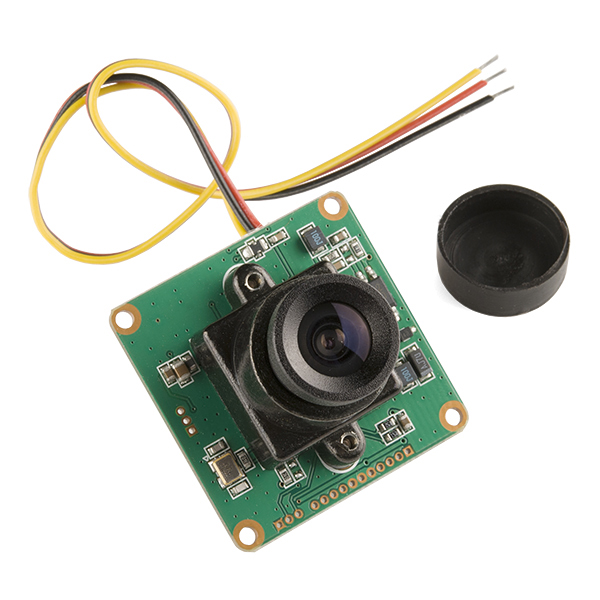
\includegraphics[width=2.0in] {Images/camera.jpg}
        \caption{Camera Module - sparkfun.com - CC BY-NC-SA 3.0}
        \label{Camera Module}
\end{figure}

\item Infrared
\\Used to detect distance from an object.  An emitter and a receiver pair linked to work like the light dependent resistor but using infrared instead of normal visible light.  Depending on the intensity of infrared picked up by the receiver it can be used to determine the distance from the source of the reflection.  Ambient infrared can effect readings as there is infrared radiation emitted from the sun and is everywhere.  This extra radiation other than the amount emitted by the sensor is unneeded and unwanted and as such if it arrives at the receiver it will provide false readings, therefore this can be very inaccurate.
\begin{figure}[H]
\centering
        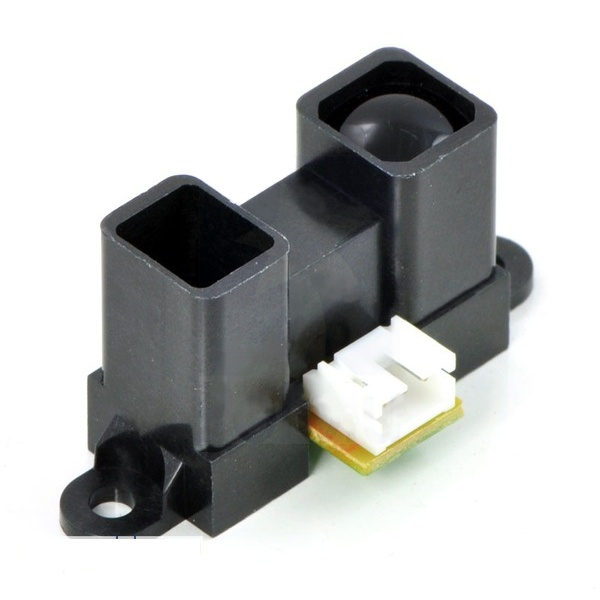
\includegraphics[width=2.0in] {Images/ir.jpg}
        \caption{Infrared Sensor - coolcomponents.co.uk}
        \label{Infrared Sensor}
\end{figure}

\item Sonar
\\An emitter style approach.  It emits an ultrasonic wave to bounce off of whatever surface is in front of it.  The time taken from emitting the wave until receiving the wave determines how far away the object is.  This method comes with its drawbacks.  Due to how sound waves behave when they interact with the environment by bouncing off of it.  If the surface is angled or curved the sound can bounce away from the receiver, either not reaching it at all giving the possible false reading that there is nothing in front of it, or it could bounce off of multiple surfaces back to the receiver giving a false reading that an object is there but further away due to the sound taking longer than it should have to reach the receiver.
\begin{figure}[H]
\centering
        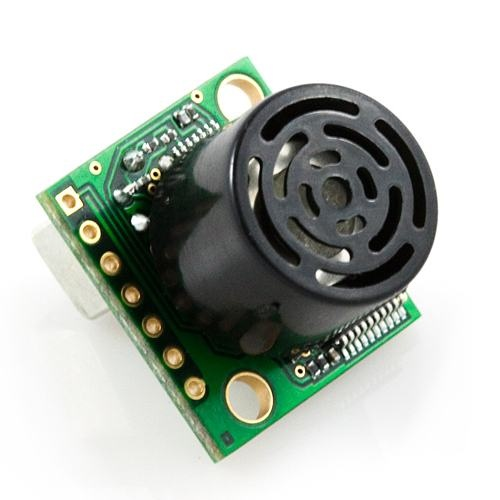
\includegraphics[width=2.0in] {Images/sonar.jpg}
        \caption{Ultrasonic Sensor - coolcomponents.co.uk}
        \label{Ultrasonic Sensor}
\end{figure}

\end{itemize}
A combination of both sonar and infrared logically seems like a good idea.  One can compensate for the others weaknesses.  Use the sonar to compensate for ambient infrared and the infrared can be used to compensate for sonar bouncing around the environment.  Hopefully this will reduce the number of false readings produced.  This does not remove the significant weaknesses of ambient infrared or the sonar echo but should help identify which readings are being affected by comparing the two different readings taken by the different sensor types.
\subsection{Control}
The robot will need a controller, that connects the software to all the hardware.
\\The ideal control unit would be:
\begin{enumerate}
\item As low power consumption as possible to increase overall total runtime of the robot.
\item As fast as possible to be able to handle any amount of processing ti may be required to do, such as analysing vast amounts of sensor data in real time.
\item As much memory as possible to be able to store all the data it will be processing as it works on it.
\item Easy to program with support for any language the user may want to write in.
\item If it to be mounted on a circuit board to be used within a larger integrated system then it should be in DIL format for easy soldering to a board via the through hole method where the legs of the chip are placed through holes in a circuit board and soldered in place.
\item Access to general purpose input and output pins, these are to interface directly with other pieces of hardware.
\end{enumerate}
If a unit like this actually existed it would be perfect but the real suitable choices are as follows.
\begin{itemize}
\item PIC
\\Peripheral Interface Controller.  Very low cost microcontroller with a small easy to learn instruction set and support serial communication/re-programming.  They also come in a DIL package (dual in-line) making them easy to incorporate into through-hole printed circuit boards as the legs of the chips can fit through these holes and be soldered (held in place with a low melting point conductive metal alloy.) into place.
\begin{figure}[H]
\centering
        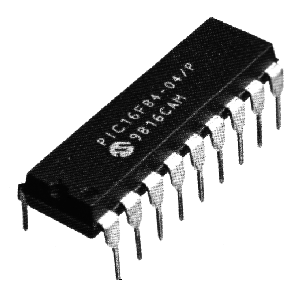
\includegraphics[width=2.0in] {Images/pic-chip.png}
        \caption{PIC - circuitstoday.com}
        \label{PIC}
\end{figure}

\item Arduino
\\An open source hardware board that is cheap but not as cheap as a PIC.  These are very popular among hobbyists due to them being very easy to use and having a vast collection of community written libraries to interface with all different types of hardware.
\\Arduino uses C or C++ programming language for development, this can be a good thing due to the fact that it provides the programmer with a large amount of control over exactly how the program runs but is more complex to use than some other languages such as python or java which handle a large amount of the low level operations for the developer.
\begin{figure}[H]
\centering
        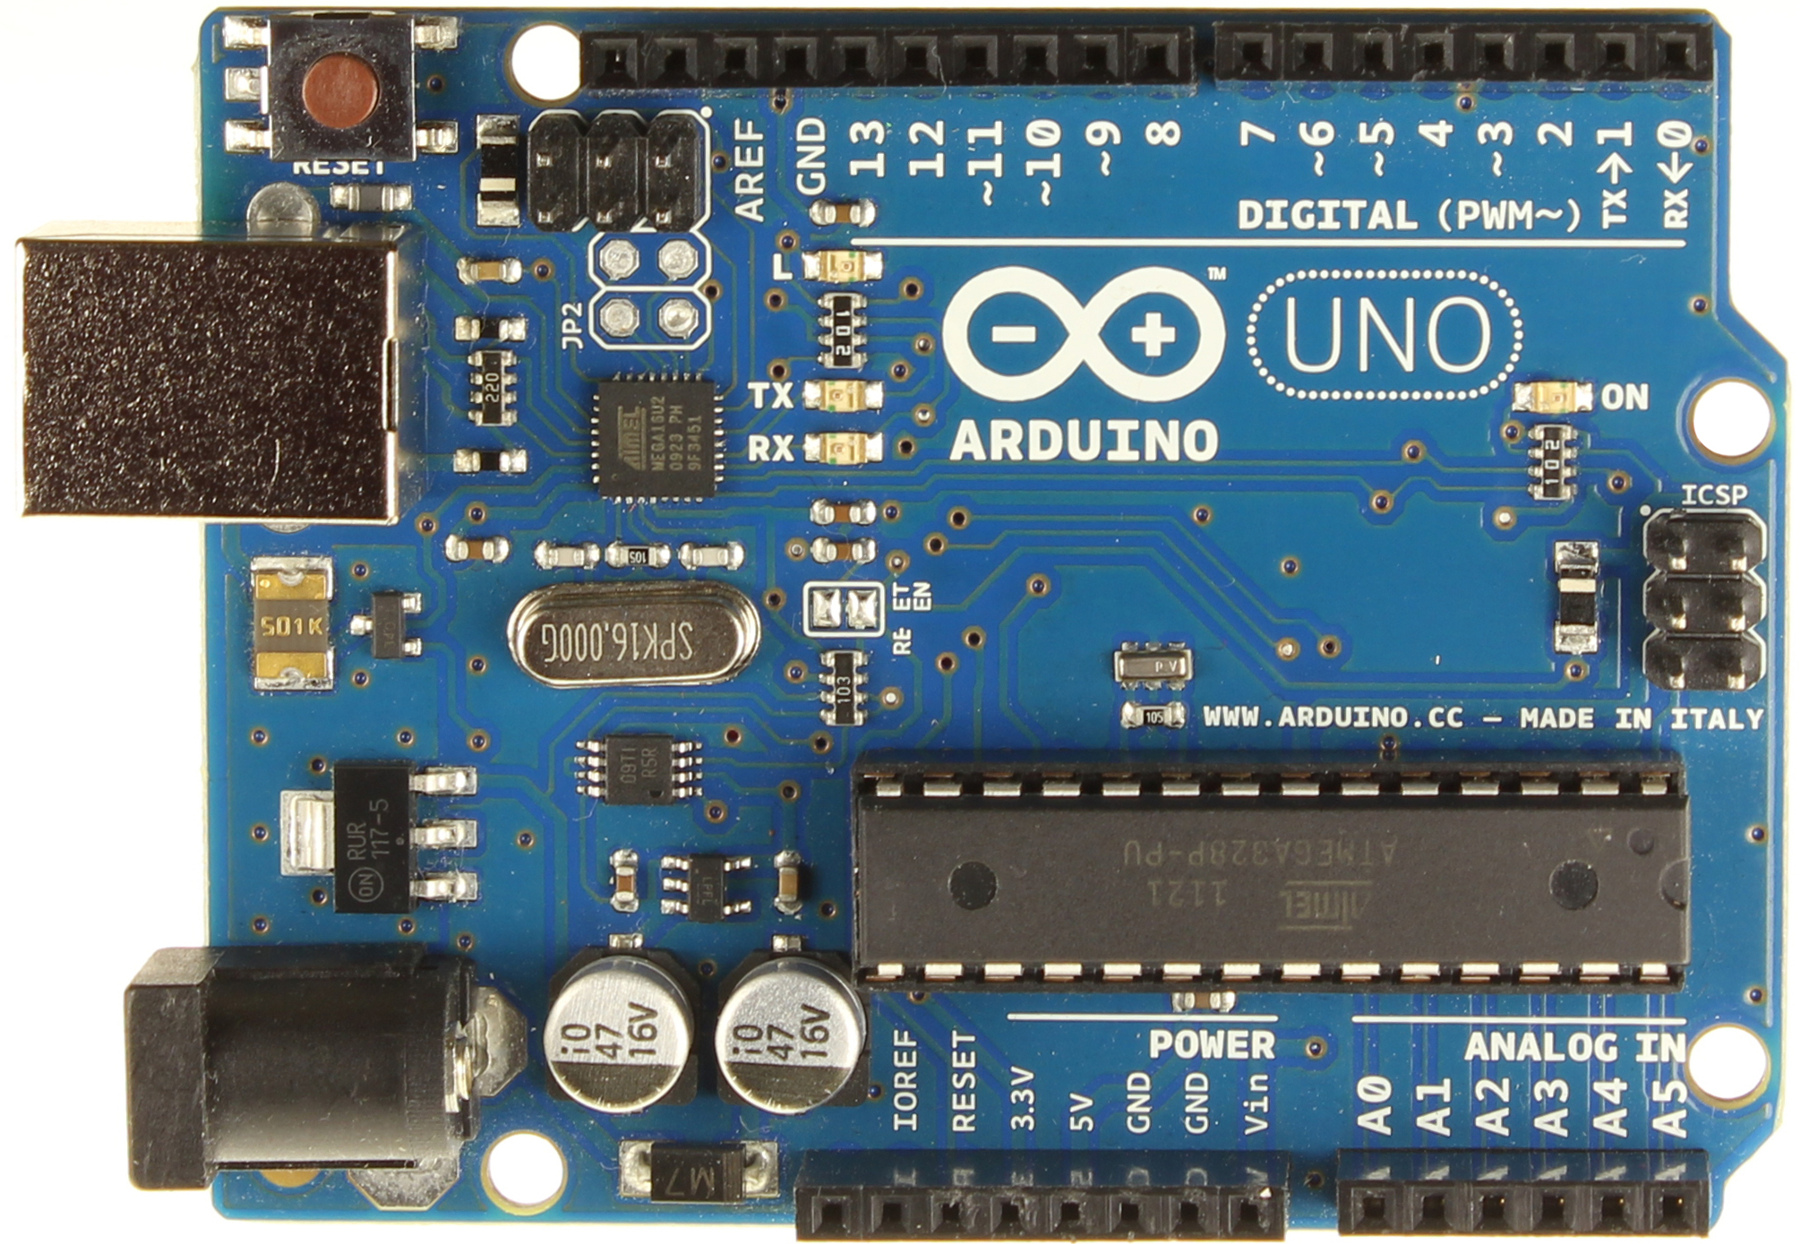
\includegraphics[width=2.0in] {Images/arduinouno-r3.jpg}
        \caption{Arduino arduino.cc}
        \label{Arduino}
\end{figure}

\item Netduino
\\This is also an open source electronics prototyping platform but instead of being based on C and C++ it is based on the .Net Micro Framework which is Microsoft's version of an embedded framework.  This could be useful to somebody who is very familiar with a .NET language such as C\#.  The main disadvantage is that this framework requires a faster processor to run and as such requires more power to operate making this option have higher overheads on power and processing than the PIC and Arduino alternatives.
\\These boards also cost more than the Arduino and PIC, and have much less community support.
\begin{figure}[H]
\centering
        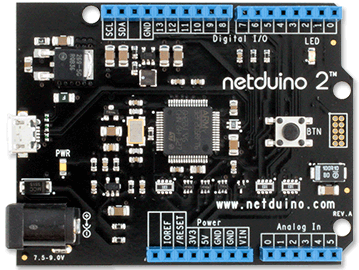
\includegraphics[width=2.0in] {Images/netduino.png}
        \caption{Netduino - netduino.com}
        \label{Netduino}
\end{figure}

\item Motherboard
\\A small motherboard that can be found in a home computer or a netbook/laptop.  These have the widest variety of applications.  It can support most operating systems and programming languages but come at the hefty price of power consumption.  Compared to microcontrollers, a full motherboard draws a very large amount of power to run.  Also they take far longer to power on due to running an operating system, unlike microcontrollers that have the code compiled down and run directly on the hardware itself.  This can also be done with these larger boards but is far more complex to do and is out of the scope of this project.
\\The cost of such boards is also very high as they are far more complex pieces of electronics.
\begin{figure}[H]
\centering
        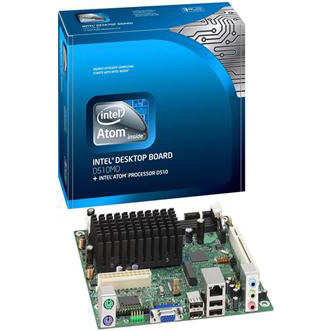
\includegraphics[width=2.0in] {Images/atom.jpg}
        \caption{Atom Motherboard - intel.co.uk}
        \label{Atom Motherboard}
\end{figure}
\item Raspberry Pi
\\The Raspberry Pi is a credit card sized computer that is an embedded platform for Linux and various other operating systems.  It is very cheap and runs much faster than most microcontrollers.  It does also have the downside of long startup times due to running a full desktop style operating system on such a compact board.  This could also be compiled to run directly on the ARM processor this board uses but is also out of the scope of this project.  Unlike normal motherboards this little board has some GPIO (general purpose input output) pins for interacting directly with various pieces of hardware like the microcontrollers do.
\begin{figure}[H]
\centering
        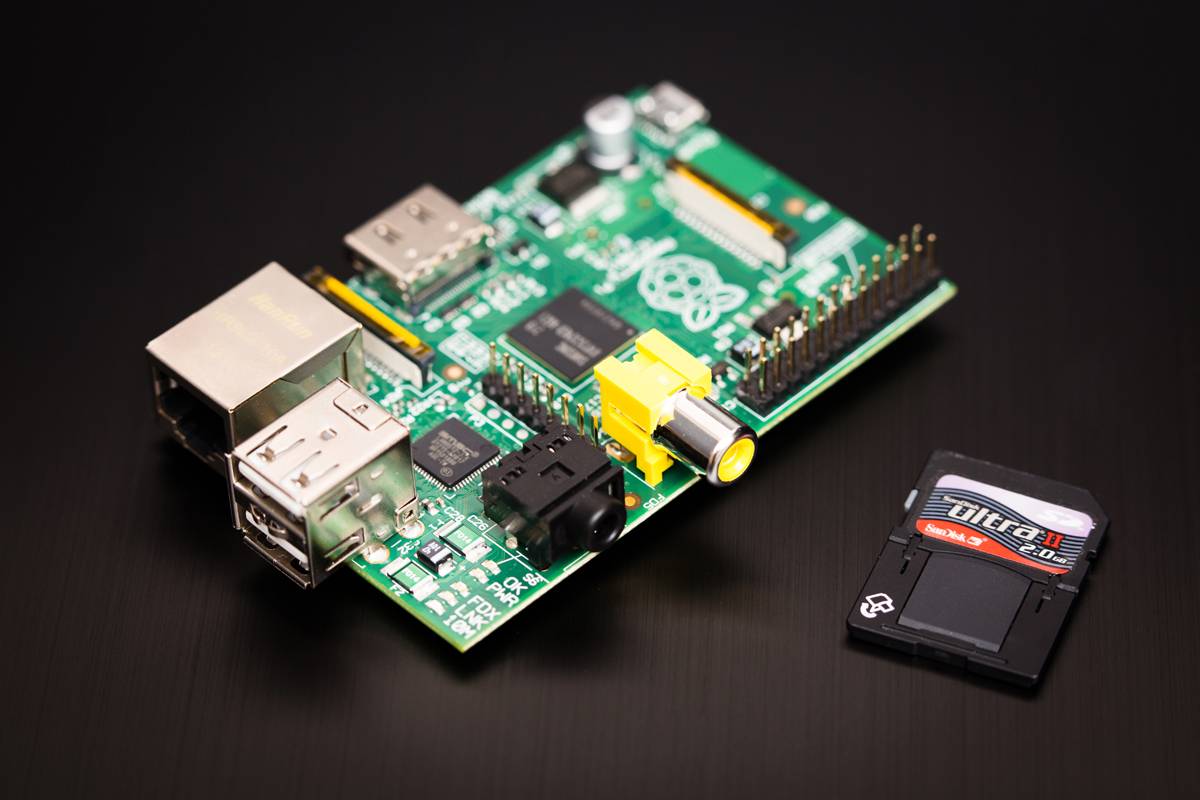
\includegraphics[width=2.0in] {Images/rpi.jpeg}
        \caption{Raspberry Pi - raspberrypi.org}
        \label{Raspberry Pi}
\end{figure}

\end{itemize}

\subsection{Power Source}
As this robot is intended to move around freely the power source should be:
\begin{enumerate}
\item Unhindered by power and data cables, the power source cannot be supplied by a wall power outlet, it has to be self contained.  This means it will have to be a battery.
\item The battery will have to be several cells or a single high output cell due to the size of motors intended.
\item It will need as many Amp hours as possible for longer run times.  This could be achieved with several cells linked together in series (end to end) to increase voltage and/or link more together in parallel (side by side) to increase amp hours (runtime).
\item It will have to be small enough to fit on the robot.
\item It should be light as to not increase the load on the drive system too much.
\end{enumerate}
The possible options are:
\begin{itemize}
\item Lithium Polymer
\\LiPo batteries come in up to 11.2 volt packages, which is not quite high enough for some higher voltage motors which I may be using such as the high end steppers.  These batteries are much lighter than some other alternatives and are common in embedded devices.  The amp hour ratings of these batteries can range from 100 milliamp hours to around typically 6 amp hours in the size packages that would be suitable for a small robot.
\begin{figure}[H]
\centering
        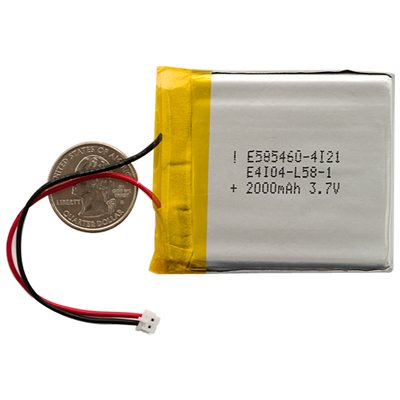
\includegraphics[width=2.0in] {Images/lipo-front.jpg}
        \caption{Lithium Polymer Battery - robotshop.com}
        \label{Lithium Polymer Battery}
\end{figure}

\item Lead Acid
\\A lead acid battery is a choice with a high output.  A single battery can output 12 volts and can be found in high amp hour packages such as 1 - 40amp hours compared to the lithium alternatives which are around 0.1 - 6 amp hours.  Due to already needing a high power motor for the chassis, a higher weight battery is not too much of an issue and provides the benefit of the higher power output to drive the more power hungry motors.
\begin{figure}[H]
\centering
        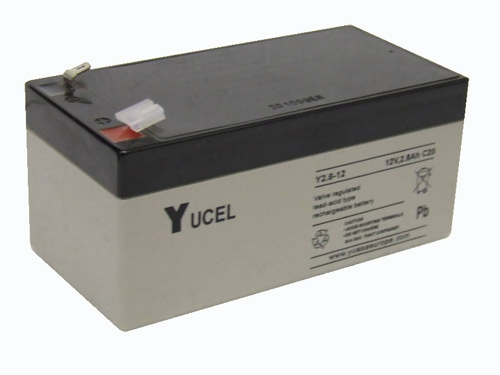
\includegraphics[width=2.0in] {Images/lead-acid.jpg}
        \caption{Lead Acid Battery - kestrelelectricalsupplies.co.uk}
        \label{Lead Acid Battery}
\end{figure}
\end{itemize}
\subsection{Wheels}
As I have chosen a wheeled solution for the drive system of the robot the wheels supporting it must be appropriate.
\\The perfect wheels would be:
\begin{enumerate}
\item Made of extremely light materials thus being easier to turn.
\item To be very strong to support all of the weight of the robot on them.
\item To have a high level of traction as not to slip on the environment it may be traversing.
\item As cheap as possible to keep overall costs to a minimum.
\item Be easy to mount to the drive shaft of the motors being used to move the wheels.
\end{enumerate}
\begin{itemize}
\item Off Road
\\Having chosen to use stepper motors for the reason of increased accuracy over the less precise DC motors it would be a bad idea to go for wheels which have insufficient traction and as such off road style wheels which have a wide and deep tread with spikes for additional grip would be a suitable solution.
\\These wheels measure 120mm in diameter and 60mm wide which results in it being harder to turn and will require a stronger motor to move.
\begin{figure}[H]
\centering
        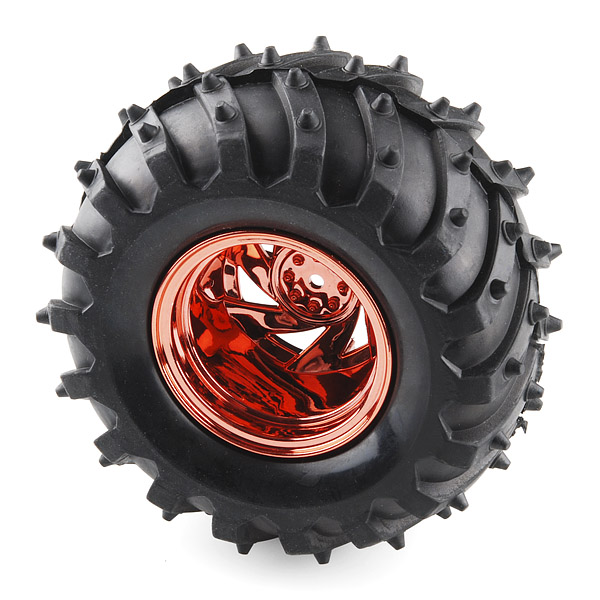
\includegraphics[width=3.0in]  {Images/wheel-offroad.jpg}
        \caption{Offroad Wheel - sparkfun.com}
        \label{Offroad Wheel}
\end{figure}

\item Colson Wheel
\\These come in sizes ranging from four inches to twelve inches in diameter with a tread width of between two and three inches.  They have a rubber exterior for grip with an iron core for mounting.  They are shock absorbent but this should not be an issue for this project due to the slow speeds that it is intended to be moving at.  The iron core makes these wheels very heavy weighing around four pounds for the smaller wheel and up to sixteen pounds for the larger versions.
\begin{figure}[H]
\centering
        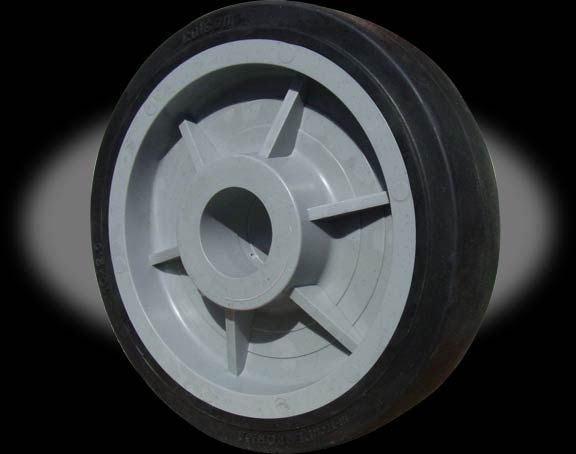
\includegraphics[width=3.0in]  {Images/colson.jpg}
        \caption{Colson Wheel - colsoncaster.com}
        \label{Colson Wheel}
\end{figure}
\item Omni Wheel
\\These wheels have been briefly described in the four wheeled drive system section but here I will go into more detail.
\\They have less grip then other wheel types due to the rollers all around the wheel.  Their primary advantage is that when two or more are used in conjunction with each other and are rotated in different directions they can move whatever device they are mounted to directly sideways, this is going against the way the wheels are actually turning.  This feature of the omni wheels is a major advantage if the robot gets stuck in a tight space that it cannot turn to get out of or even just a tight turn that it's normal turning circle is not sufficient to traverse.
\begin{figure}[H]
\centering
        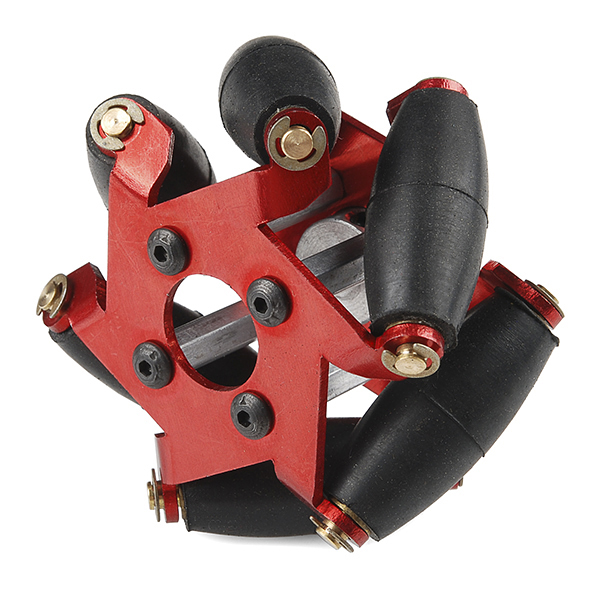
\includegraphics[width=3.0in] {Images/mechanum.jpg}
        \caption{Omni Wheel - sparkfun.com}
        \label{Omni Wheel}
\end{figure}

\end{itemize}
\section{Feedback Interface}
While operating the robot, if there is any unexpected behaviour it would be nice to have some form of interface to see what the robot thinks the environment looks like.
\\An ideal solution for this should conform to the following guidelines:
\begin{enumerate}
\item There cannot be any cables trailing from the robot to the feedback device because you do not want to have to follow the robot around it's environment just to be able to read what it thinks it is seeing, so a wireless solution would be good.
\item Be lightweight so that carrying it is not a nuisance.
\item Low power consumption so that it does not need to be near a power source all the time.  Having a run time the same as or longer than the robot itself would be ideal.
\item Easy to read display which is also low power.
\item Intuitive user interface so that it is very easy to use and enables the user to just use it without any instruction.
\end{enumerate}
All that is needed is a small microcontroller as learned from the previous sections that these are low powered, easy to use and have support for various different pieces of hardware.
\\Lithium ion batteries are a good fit for this sort of device due to their low weight, low voltage and small size.
\\A small display is needed.
\begin{itemize}
\item Liquid Crystal Display
\\These are low powered easy to use devices for displaying information.  They are used in everyday machines such as a digital display on an oven or microwave, the screen on a calculator or a vending machine even the screens used in mobile telephones.  These screens are very cheap and easily available in all sorts of types and sizes.
\begin{figure}[H]
\centering
        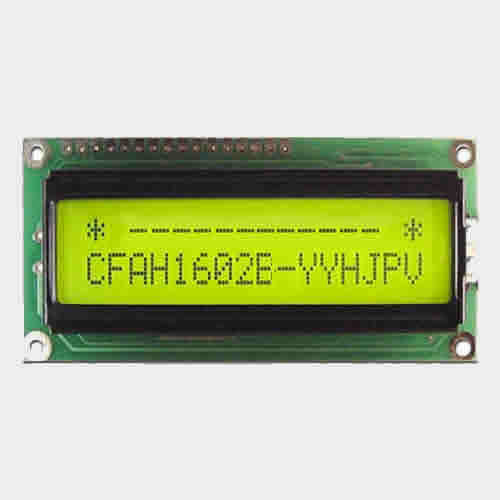
\includegraphics[width=2.0in] {Images/lcd.jpg}
        \caption{Liquid Crystal Display - coolcomponents.co.uk}
        \label{Liquid Crystal Display}
\end{figure}
\item E-Ink Display
These displays are unique in that they only use power to change what they are displaying, once the display has changed it used no more energy to keep the screen displaying it's current image.  The main downside to these is getting hold of one that has not been removed from another device such as an e-reader.  Some of these displays are also flexible and could be used to wrap around the wrist as a type of watch display.  They are also very expensive for a simple display but the power consumption aspect makes them a very attractive option for this type of device.
\begin{figure}[H]
\centering
        
\includegraphics[width=4.0in] {Images/e-ink-display.png}
        \caption{E-Ink Display - dataprotectioncenter.com}
        \label{E-Ink Display}
\end{figure}
\end{itemize}
A wireless module of some description will be needed to transmit the information from the robot to the feedback device.  This device should ideally conform to these guidelines:
\begin{enumerate}
\item Have as much range as possible so that no matter how far away the robot goes it can still receive the information from it.
\item Be able to transmit through any material so that no matter what obstacles get between the robot and the feedback device it can still receive information.
\item Consume as little amount of power as possible to increase the run time of the device.
\item Be physically small to keep the size of the device as small as possible.
\item Be as light as possible to keep the overall device weight to a minimum for comfort as the user may be holding it for prolonged periods of time.
\end{enumerate}
The options for this type of component are:
\begin{itemize}
\item Wifi
\\This is the most common wireless medium for transmitting large amounts of data.  It has some low powered modules with a consumption rate of only 100 milliwatts and this low power module can transmit data at 1Mbps (mega bits per second).  The downside is that these low power versions are expensive costing around fifty dollars a piece.
\begin{figure}[H]
\centering
        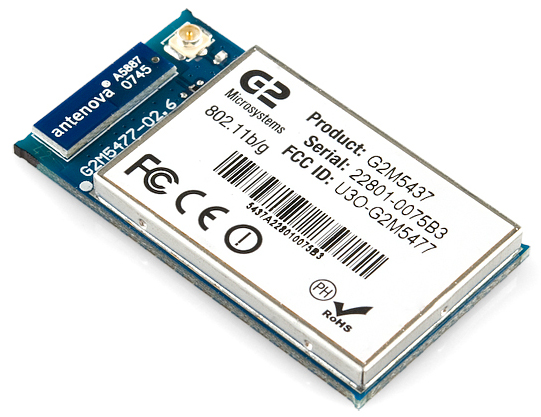
\includegraphics[width=2.0in] {Images/wifi-module.jpg}
        \caption{Wifi Module - antenova-m2m.com}
        \label{Wifi Module}
\end{figure}
If a USB connection is available with a host that has the appropriate drivers to run a USB wifi module then a cheaper version is available at around fifteen dollars but these have a much higher processing overhead for any device that is capable of using such a module which in turn uses more power.  The module itself is still around 100-500 milliwatts of power usage.
\begin{figure}[H]
\centering
        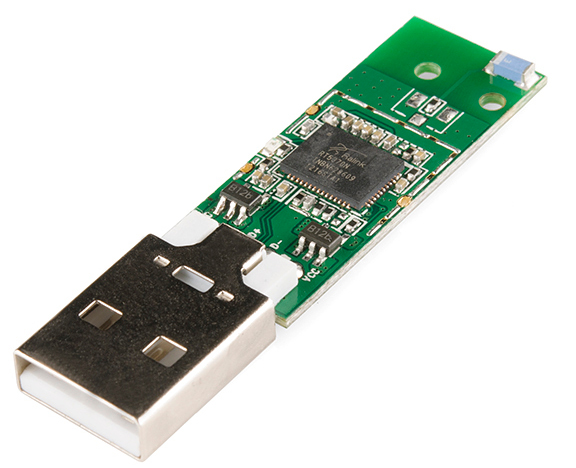
\includegraphics[width=2.0in] {Images/usb-wifi.jpg}
        \caption{USB Wifi - sparkfun.com}
        \label{Usb Wifi}
\end{figure}
Both of the Wifi module types have a maximum range of around one hundred meters.

\item Bluetooth
This type of communication is commonly using in mobile telephones to enable such things as hands free calls in an automobile.  Low power Bluetooth units that transmit data at around 1200 bits per second typically use only 24 milliwatts of power in doing so.  This is much lower than the low power version of wifi but it has severe range limitations of only being reliable within 10-20 meters.  The Bluetooth modules available for use in hobbyist projects such as this are rather pricey costing around forty dollars each.
\begin{figure}[H]
\centering
        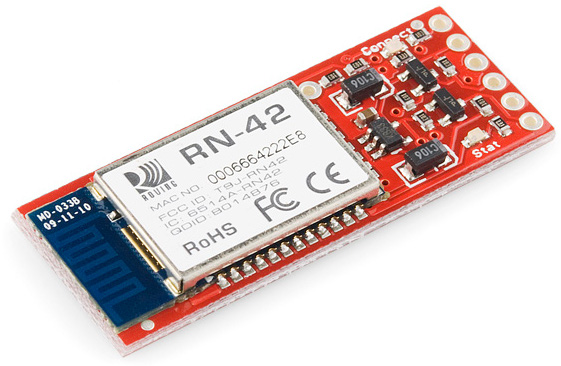
\includegraphics[width=2.0in] {Images/bluetooth.jpg}
        \caption{Bluetooth Module - sparkfun.com}
        \label{Bluetooth Module}
\end{figure}
\item Zigbee
These little wireless radios are perfect for small, low powered wireless projects.  They run on as little as 3.3 volts with an output of 1 milliwatt.  The downside is that it's data transfer rate is only around 250 killobits per second, just a quarter of the embedded wifi module.  The zigbee module more than makes up for the lack of data transfer with its increased range of up to 100 meters.  These are also one of the cheaper options costing around twenty dollars each.  These such modules are called xbee which is just an implementation of the zigbee protocol which is typically used for mesh networking but still works for single point to point communications.
\end{itemize}
An Arduino Fio is a good fit as it is small, low powered, has both lithium polymer battery socket and an xbee wireless module socket built in making it the obvious choice for this type of device as most of the connection work has been done already just leaving the screen and a user input method to be added.
\\A small LCD (liquid crystal display) can be connected to the Arduino to display information it receives over the integrated xbee socket.
\\A user input interface can be added by using some small push buttons and wiring them to some of the input pins provided on the Arduino Fio.

